\chapter{Bài 4. Chuyển động thẳng}
\begin{center}
	\textit{(6 tiết)}
\end{center}
\section{MỤC TIÊU DẠY HỌC}
\begin{center}
	\begin{longtable}{|M{2.5cm}|L{12.5cm}|M{2cm}|}
		\hline
		\thead{Biểu hiện\\ năng lực} & \thead{Mục tiêu} & \thead{STT}\\
		\hline
		\multicolumn{3}{|c|}{\textbf{ Năng lực vật lí}}\\
		
		\hline
		1.1& Từ hình ảnh hoặc ví dụ thực tiễn, định nghĩa được độ dịch chuyển. & 1\\
		\hline
		1.3 & So sánh được quãng đường đi được và độ dịch chuyển. &2\\
		\hline
		1.2 & Lập luận để rút ra được công thức tính tốc độ trung bình, định nghĩa được tốc độ theo một phương. & 3\\
		\hline
		1.4 & Dựa vào định nghĩa tốc độ theo một phương và độ dịch chuyển, rút ra được công thức tính và định nghĩa được vận tốc. & 4\\
		\hline
		1.2 &  Dựa trên số liệu cho trước, vẽ được đồ thị độ dịch chuyển – thời gian trong chuyển động thẳng.& 5\\
		\hline
		1.2 & Tính được tốc độ từ độ dốc của đồ thị độ dịch chuyển – thời gian. & 6\\
		\hline
		\hline
		1.2 & Vận dụng được công thức tính tốc độ, vận tốc. & 7\\
		\hline
		\multicolumn{3}{|c|}{\textbf{Năng lực chung}}\\
		\hline
		TC - TH& Tích cực thực hiện các nhiệm vụ GV đặt ra cho các nhóm, tích cực suy luận để đưa ra câu trả lời trong quá trình GV định hướng nội dung học tập	&8 \\
		\hline
		GT - HT & Tích cực đóng góp ý kiến trong quá trình thảo luận, biết sử dụng ngôn ngữ kết hợp với các loại phương tiện phi ngôn ngữ đa dạng để trình bày các kết quả thảo luận nhóm & 10\\
		\hline
	\end{longtable}
\end{center}
\section{THIẾT BỊ DẠY HỌC VÀ HỌC LIỆU}
\begin{itemize}
	\item Tivi/máy chiếu;
	\item SGK;
	\item Phiếu học tập.
\end{itemize}
\section{TIẾN TRÌNH DẠY HỌC}
\subsection{TIẾN TRÌNH}\newpage
\begin{center}
	\begin{longtable}{|L{2.75cm}|C{1.25cm}|L{5cm}|L{3.5cm}|L{4cm}|}
		\hline
		\thead{Tiến trình} & \thead{Mục\\tiêu} & \thead{Nội dung dạy học \\trọng tâm} & \thead{PP,\\ KTDH} & \thead{Phương pháp \\đánh giá}\\
		\hline
	\textbf{Hoạt động 1:} Phân biệt khái niệm quãng đường và độ dịch chuyển	&1, 2  & Phân biệt khái niệm quãng đường và độ dịch chuyển  & PPDH: Đàm thoại& GV đánh giá dựa trên câu trả lời của HS.\newline
	PP đánh giá: quan sát, nghe. \\
		\hline
		\textbf{Hoạt động 2:} Tìm hiểu khái niệm tốc độ	& 3  & Khái niệm và công thức tính tốc độ trung bình, tốc độ tức thời  & PPDH:  Đàm thoại\newline KTDH: Động não& GV đánh giá dựa trên câu trả lời của HS.\newline
		PP đánh giá: quan sát, nghe. \\
		\hline
		\textbf{Hoạt động 3:} Tìm hiểu khái niệm vận tốc	& 4  & Khái niệm và công thức tính vận tốc trung bình, vận tốc tức thời  & PPDH:  Đàm thoại\newline KTDH: Động não& GV đánh giá dựa trên câu trả lời của HS.\newline
		PP đánh giá: quan sát, nghe. \\
		\hline
		\textbf{Hoạt động 4:} Tìm hiểu đồ thị độ dịch chuyển - thời gian	& 5, 6, 8, 10  & Vẽ đồ thị độ dịch chuyển - thời gian từ số liệu cho trước, cách xác định tốc độ tức thời từ đồ thị độ dịch chuyển - thời gian  & PPDH:  Dạy học hợp tác& GV đánh giá dựa trên câu trả lời của HS và kết quả thảo luận nhóm.\newline
		PP đánh giá: quan sát, nghe. \\
		\hline
		\textbf{Hoạt động 5:} Luyện tập	& 6, 7  & Luyện tập tính tốc độ trung bình, vận tốc trung bình trong chuyển động thẳng, từ số liệu cho trước vẽ được đồ thị độ dịch chuyển - thời gian, tính tốc độ tức thời và vận tốc tức thời từ đồ thị độ dịch chuyển - thời gian. & PPDH:  Đàm thoại& GV đánh giá dựa trên bài tập cá nhân của học sinh.\newline
		PP đánh giá: quan sát, nghe. \\
		\hline
	\end{longtable}
\end{center}
\subsection{CÁC HOẠT ĐỘNG HỌC}
% ==========================================================================================
\hoatdong
{
	Tìm hiểu đồ thị độ dịch chuyển - thời gian
}
{\begin{itemize}
		\item HS định nghĩa được độ dịch chuyển.
		\item  HS so sánh được quãng đường đi được và độ dịch chuyển.
	\end{itemize}
	
}
{
	Kết quả trả lời của HS cho các câu hỏi gợi mở của GV:\\
	\textbf{Câu trả lời dự kiến:} 
	\begin{itemize}
		\item Trường hợp nhân vật đi từ O đến B:
		\begin{itemize}
			\item quãng đường đi là $s=OB$;
			\item độ dịch chuyển là $d=OB$.
		\end{itemize}
		\item Trường hợp nhân vật đi từ O đến B rồi về A:
		\begin{itemize}
			\item quãng đường đi là $s=OB+AB$;
			\item độ dịch chuyển là $d=OA$.
		\end{itemize}
	\end{itemize}
}
{\textit{\underline{* GV chuyển giao nhiệm vụ học tập}}\\
	GV giới thiệu cho học sinh về khái niệm quãng đường và độ dịch chuyển.\\
	GV yêu cầu HS xác định độ dịch chuyển và quãng đường đi được của nhân vật trong ví dụ hình bên trong các trường hợp
	\begin{center}
		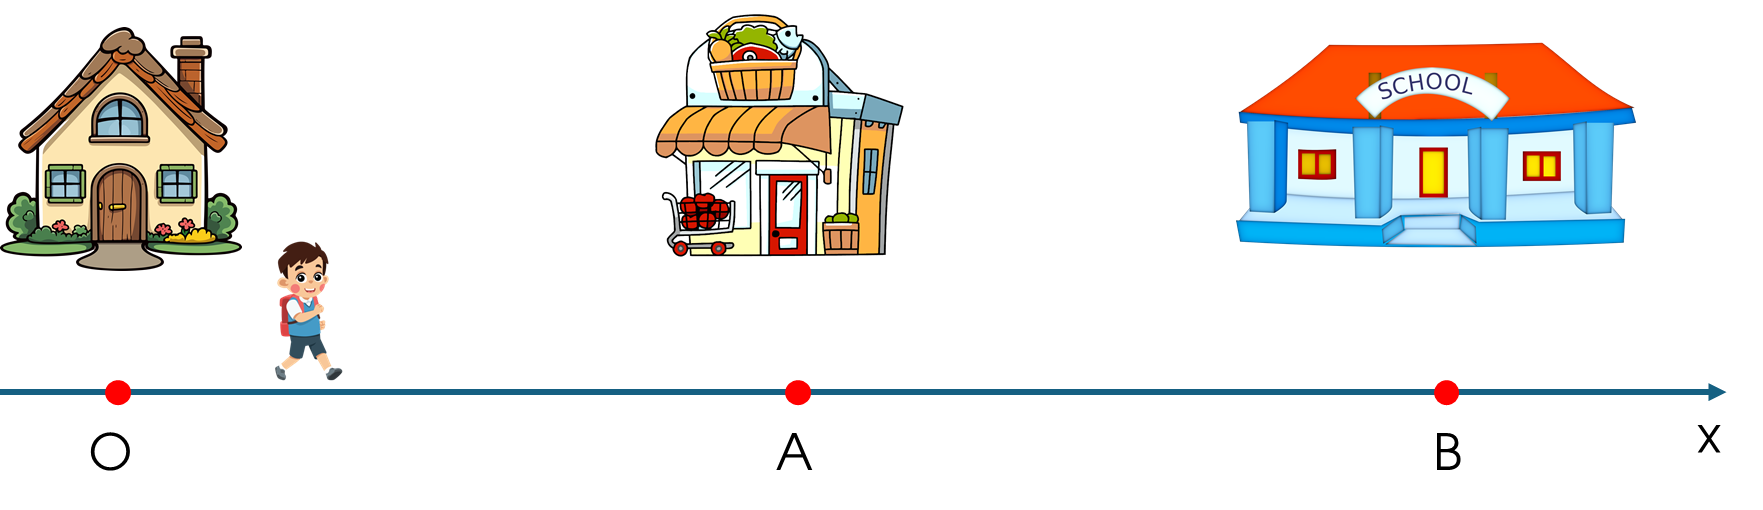
\includegraphics[width=0.9\linewidth]{figs/BAI4-1}
	\end{center}
	\begin{itemize}
		\item nhân vật đi từ nhà đến trường.
		\item nhân vật đi từ nhà đến trường rồi đến cửa hàng tạp hóa.
	\end{itemize}
	\textit{\underline{* HS thực hiện nhiệm vụ học tập}}\\
	HS tích cực trả lời câu hỏi gợi mở của GV.\\
	HS chú ý theo dõi, đặt câu hỏi.
}
% ==========================================================================================
\hoatdong
{
	Tìm hiểu khái niệm tốc độ
}
{\begin{itemize}
		\item HS nêu được tốc độ là đại lượng đặc trưng cho tính chất nhanh, chậm của chuyển động.
		\item HS lập luận rút ra được công thức tính tốc độ trung bình.
	\end{itemize}
	
}
{
	Kết quả trả lời của HS cho các câu hỏi gợi mở của GV:\\
	\textbf{Câu trả lời dự kiến:} Trung bình 1 giây vận động viên bơi được $\SI{2}{\meter}$ ở lần đầu và $\SI{1.79}{\meter}$ ở lần sau. Như vậy, lần đầu vận động viên này bơi nhanh hơn.
}
{\textit{\underline{* GV chuyển giao nhiệm vụ học tập}}\\
GV đặt ra tình huống để HS thảo luận theo nhóm đôi:\\
\textit{Một vận động viên bơi lội người Mỹ đã từng lập kỉ lục thế giới ở nội dung bơi bướm $\SI{100}{\meter}$ và $\SI{200}{\meter}$ với thời gian lần lượt là $\SI{49.82}{\second}$ và $\SI{111.51}{\second}$. Hãy lập luận để xác định vận động viên này bơi nhanh hơn trong trường hợp nào?}\\
Từ câu trả lời của HS, GV dẫn dắt đến khái niệm tốc độ trung bình.\\
GV giới thiệu cho HS khái niệm tốc độ tức thời.\\
GV đặt câu hỏi: \textit{Vậy số chỉ trên tốc kế là tốc độ trung bình hay tốc độ tức thời?}\\
\textit{\underline{* HS thực hiện nhiệm vụ học tập}}\\
HS tích cực trả lời câu hỏi gợi mở của GV.\\
HS chú ý theo dõi, đặt câu hỏi.\\
\textit{\underline{* HS báo cáo kết quả thực hiện nhiệm vụ học tập}}\\
GV lần lượt mời 1 HS trả lời câu hỏi và 1 HS khác nhận xét câu trả lời.\\
HS theo dõi, nhận xét, đặt câu hỏi.\\
GV chỉnh lí, hợp thức hoá kiến thức.
}
% ==========================================================================================
\hoatdong
{
	Tìm hiểu khái niệm vận tốc
}
{\begin{itemize}
		\item HS dựa vào định nghĩa tốc độ theo một phương và độ dịch chuyển, rút ra được công thức tính và định nghĩa được vận tốc.
		\item HS phân biệt được tốc độ trung bình và vận tốc trung bình.
	\end{itemize}

}
{
	Câu trả lời của HS cho câu hỏi gợi mở do GV đưa ra:\\
	\textbf{Câu trả lời dự kiến:} Cần phải biết thêm hướng chuyển động của hai người mới có thể xác định được vị trí gặp nhau.
}
{\textit{\underline{* GV chuyển giao nhiệm vụ học tập}}\\
	GV đặt câu hỏi gợi mở: \textit{Có hai người đi xe máy khởi hành cùng lúc từ thành phố A và thành phố B cách nhau $\SI{40}{\kilo\meter}$ với tốc độ không đổi $\SI{40}{\kilo\meter/\hour}$ và $\SI{60}{\kilo\meter/\hour}$ trên một đường thẳng. Em có thể xác định được thời điểm hai người gặp nhau không? Vì sao?}\\
	Từ câu trả lời của HS, GV rút ra kết luận: \textit{Tốc độ không cho biết hướng chuyển động. Trong các bài toán khảo sát vị trí của vật, ta cần quan tâm đến độ dịch chuyển của vật theo thời gian. Thay đại lượng $s$ trong công thức tốc độ trung bình bằng độ dịch chuyển $\vec{d}$ ta có được đại lượng mới, được gọi là vận tốc trung bình $\vec{v}_{\text{tb}}=\dfrac{\vec{d}}{\Delta t}=\dfrac{\Delta \vec{x}}{\Delta t}$.}\\
	GV đặt câu hỏi để đi đến phần lưu ý: \textit{Vậy khi nào thì tốc độ trung bình bằng với độ lớn của vận tốc trung bình?}\\
	GV giới thiệu khái niệm vận tốc tức thời.\\
	\textit{\underline{* HS thực hiện nhiệm vụ học tập}}\\
	HS tích cực trả lời câu hỏi gợi mở của GV.\\
	HS chú ý theo dõi, đặt câu hỏi.\\
	\textit{\underline{* HS báo cáo kết quả thực hiện nhiệm vụ học tập}}\\
	GV lần lượt mời 1 HS trả lời câu hỏi và 1 HS khác nhận xét câu trả lời.\\
	HS theo dõi, nhận xét, đặt câu hỏi.\\
	GV chỉnh lí, hợp thức hoá kiến thức.
}
% ==========================================================================================
\hoatdong
{
	Tìm hiểu đồ thị độ dịch chuyển - thời gian
}
{\begin{itemize}
		\item HS vẽ được đồ thị độ dịch chuyển - thời gian từ số liệu cho trước.
		\item HS xác định được tốc độ tức thời, vận tốc tức thời từ đồ thị độ dịch chuyển - thời gian.
	\end{itemize}
	
}
{
	Kết quả thảo luận nhóm của HS.
}
{\textit{\underline{* GV chuyển giao nhiệm vụ học tập}}\\
	GV ôn tập lại cho HS phần đồ thị hàm số bậc nhất, nội dung ôn tập như sau:
	\begin{itemize}
		\item Đồ thị hàm số $y=ax+b\ \left(a\neq0\right)$ là đường thẳng.
		\item Hệ số góc của đường thẳng $a=\tan\beta=\dfrac{\Delta y}{\Delta x}=\dfrac{y_{\mathrm{B}}-y_{\mathrm{A}}}{x_{\mathrm{B}}-x_{\mathrm{A}}}.$
	\end{itemize}
	\begin{center}
		\begin{tabular}{M{8cm}M{8cm}}
			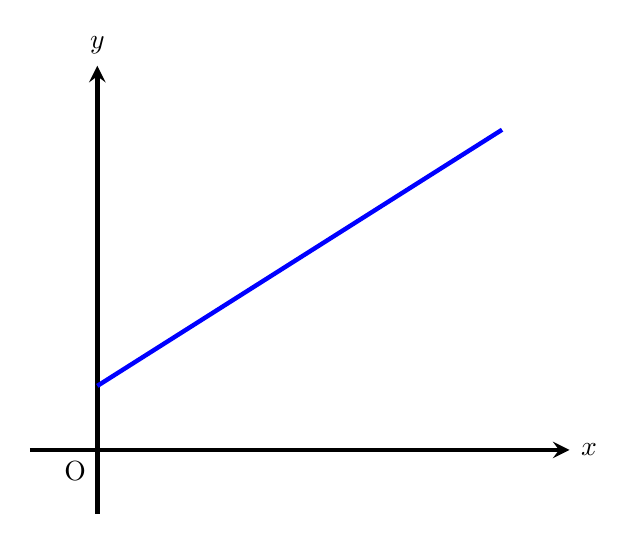
\begin{tikzpicture}  
				\begin{axis}[  ultra thick,
					xmin=-1,  
					xmax=7,  
					ymin=-1,  
					ymax=6, 
					samples=300,
				xtick=\empty,
				ytick=\empty,
					yticklabels=\empty,
					xticklabels=\empty,
					axis lines=center, 
					xlabel=$x$, 		ylabel=$y$,
					every axis y label/.style={at=(current axis.above origin),anchor=south},  
					every axis x label/.style={at=(current axis.right of origin),anchor=west},  ]
					\addplot [ultra thick, blue, smooth, domain=0:6] {1+2*x/3};
					\node[below left] at (axis cs: 0, 0) {O}; 
				\end{axis}  
			\end{tikzpicture} &
			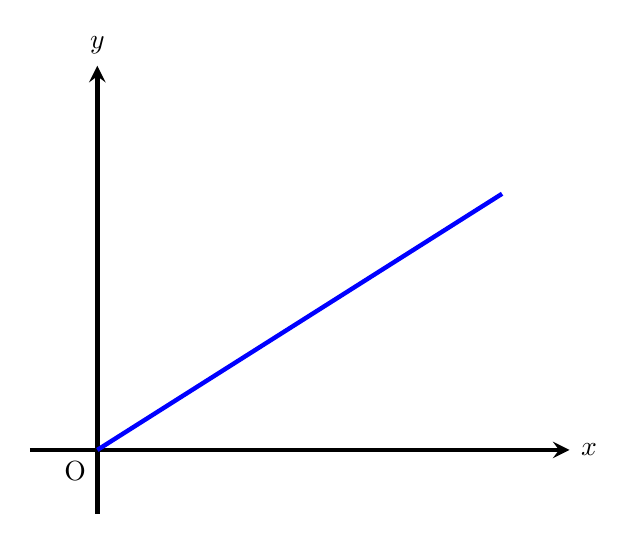
\begin{tikzpicture}  
				\begin{axis}[  ultra thick,
					xmin=-1,  
					xmax=7,  
					ymin=-1,  
					ymax=6, 
					xtick=\empty,
					ytick=\empty,
					samples=300,
					yticklabels=\empty,
					xticklabels=\empty,
					axis lines=center, 
					xlabel=$x$, 		ylabel=$y$,
					every axis y label/.style={at=(current axis.above origin),anchor=south},  
					every axis x label/.style={at=(current axis.right of origin),anchor=west},  ]
					\addplot [ultra thick, blue, smooth, domain=0:6] {2*x/3}; 
					\node[below left] at (axis cs: 0, 0) {O};
				\end{axis}  
			\end{tikzpicture}\\
			$b\neq 0$ & $b=0$
		\end{tabular}
	\end{center}
	\begin{center}
		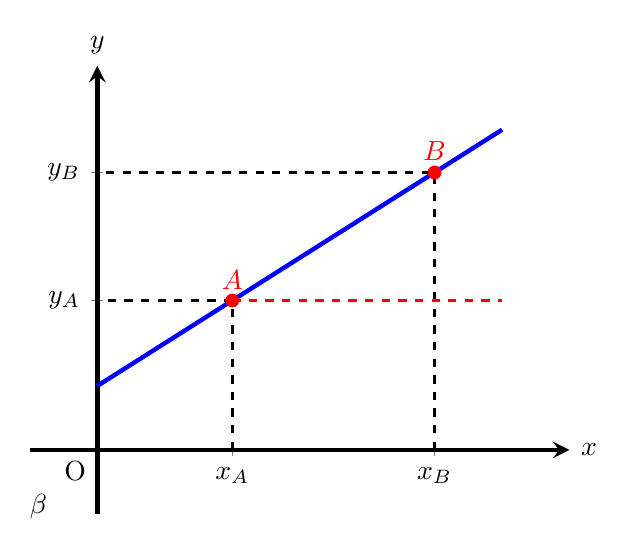
\begin{tikzpicture}  
			\begin{axis}[  ultra thick,
				xmin=-1,  
				xmax=7,  
				ymin=-1,  
				ymax=6, 
				samples=300,
				xtick={2, 5},
				ytick={2.3333, 4.3333},
				yticklabels={$y_A$, $y_B$},
				xticklabels={$x_A$, $x_B$},
				axis lines=center, 
				xlabel=$x$, 		ylabel=$y$,
				every axis y label/.style={at=(current axis.above origin),anchor=south},  
				every axis x label/.style={at=(current axis.right of origin),anchor=west},  ]
				\coordinate (A) at (axis cs: 2, 2.3333);
				\coordinate (B) at (axis cs: 5, 4.3333);
				\coordinate (C) at (axis cs: 6, 2.3333);
				\addplot [ultra thick, blue, smooth, domain=0:6] {1+2*x/3};
				\node[below left] at (axis cs: 0, 0) {O}; 
				\draw[dashed, line width=1pt] (axis cs: 2,0)--(A)--(axis cs:0,2.3333);
				\draw[dashed, line width=1pt] (axis cs: 5,0)--(B)--(axis cs:0,4.3333);
				\draw[dashed, line width=1pt, red] (A)--(axis cs:6,2.3333);
				\fill[red]   (A) circle[radius=2.5pt]  node [above] {$A$};
				\fill[red]   (B) circle[radius=2.5pt]  node [above] {$B$};
			\end{axis} 
			\tkzMarkAngle[size=0.75cm,color=red, line width=1pt](C,A,B);
			\tkzLabelAngle[color=black,pos=1.2](C,A,B){$\beta$}; 
		\end{tikzpicture}
		
	\end{center}
	\begin{itemize}
		\item Hệ số góc $a$ càng lớn thì góc $\beta$ càng lớn (đồ thị càng dốc).
	\end{itemize}
GV hướng dẫn HS xây dựng phương trình tọa độ của vật chuyển động thẳng đều:
\begin{itemize}
	\item Chất điểm chuyển động thẳng đều: 
	$$v=\dfrac{d}{\Delta t}=const\Rightarrow d=v\Delta t=v\left(t-t_0\right).$$
	\item Nếu chọn gốc thời gian lúc vật qua gốc toạ độ $(t_0=0)$, thì phương trình độ dịch chuyển của chất điểm so với gốc toạ độ: $d=v\cdot t$.\\
	Như vậy, đồ thị độ dịch chuyển thời gian của vật chuyển động thẳng đều là 1 đường thẳng:
	\begin{center}
		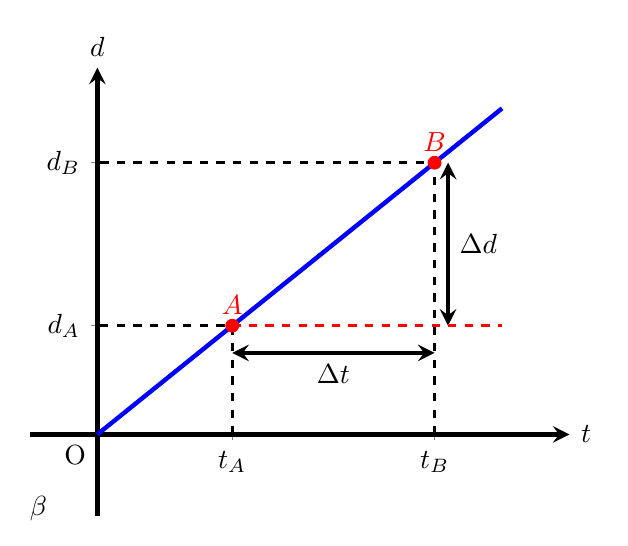
\begin{tikzpicture}  
			\begin{axis}[  ultra thick,
				xmin=-1,  
				xmax=7,  
				ymin=-1,  
				ymax=4.5, 
				samples=300,
				xtick={2, 5},
				ytick={1.3333, 3.3333},
				yticklabels={$d_A$, $d_B$},
				xticklabels={$t_A$, $t_B$},
				axis lines=center, 
				xlabel=$t$, 		ylabel=$d$,
				every axis y label/.style={at=(current axis.above origin),anchor=south},  
				every axis x label/.style={at=(current axis.right of origin),anchor=west},  ]
				\coordinate (A) at (axis cs: 2, 1.3333);
				\coordinate (B) at (axis cs: 5, 3.3333);
				\coordinate (C) at (axis cs: 6, 1.3333);
				\draw[stealth-stealth] (axis cs: 2,1)--(axis cs: 5,1);
				\draw[stealth-stealth] (axis cs: 5.2,3.3333)--(axis cs: 5.2,1.3333);
				\addplot [ultra thick, blue, smooth, domain=0:6] {2*x/3};
				\node[below left] at (axis cs: 0, 0) {O}; 
				\draw[dashed, line width=1pt] (axis cs: 2,0)--(A)--(axis cs:0,1.3333);
				\draw[dashed, line width=1pt] (axis cs: 5,0)--(B)--(axis cs:0,3.3333);
				\draw[dashed, line width=1pt, red] (A)--(axis cs:6,1.3333);
				\fill[red]   (A) circle[radius=2.5pt]  node [above] {$A$};
				\fill[red]   (B) circle[radius=2.5pt]  node [above] {$B$};
				\node[below] at (axis cs: 3.5, 1) {$\Delta t$};
				\node[right] at (axis cs: 5.2, 2.3333) {$\Delta d$};
			\end{axis} 
			\tkzMarkAngle[size=0.75cm,color=red, line width=1pt](C,A,B);
			\tkzLabelAngle[color=black,pos=1.2](C,A,B){$\beta$}; 
		\end{tikzpicture}
		
	\end{center}
	\begin{itemize}
		\item Độ dốc của đồ thị $d\left(t\right)$ càng lớn, vật chuyển động càng nhanh (tốc độ càng lớn): $v=\tan\beta=\dfrac{\Delta d}{\Delta t}=\dfrac{d_{\mathrm{B}}-d_{\mathrm{A}}}{t_{\mathrm{B}}-t_{\mathrm{A}}}$.
		\item Nếu hệ số góc của đồ thị $d\left(t\right)$ âm, vật đang chuyển động ngược chiều dương.
	\end{itemize}
\end{itemize}
GV yêu cầu HS thảo luận nhóm đôi để thực hiện ví dụ 1 trong thời gian 15 phút, sau 15 phút GV mời đại diện của 1 nhóm HS bất kì lên bảng giải bài.\\
GV dẫn dắt HS từ phương trình độ dịch chuyển - thời gian của vật chuyển động thẳng đều suy ra phương trình tọa độ - thời gian của vật chuyển động thẳng đều:
 $$d=x-x_0=vt\Rightarrow x=x_0+vt.$$
 GV dùng kĩ thuật tia chớp, yêu cầu HS thực hiện ví dụ 2, HS có kết quả nhanh nhất sẽ lên bảng giải bài và nhận được 1 điểm cộng.\\
 GV yêu cầu HS thảo luận nhóm đôi để thực hiện ví dụ 3. Sau 15 phút, GV mời đại diện 1 nhóm HS lên bảng trình bày kết quả. \\
 \textit{\underline{* HS thực hiện nhiệm vụ học tập}}\\
 HS theo dõi, tích cực trả lời câu hỏi của GV.\\
 HS thảo luận nhóm đôi để thực hiện ví dụ 1 và ví dụ 3.\\
 HS làm việc cá nhân để thực hiện ví dụ 2.\\
 \textit{\underline{* HS báo cáo kết quả thực hiện nhiệm vụ học tập}}\\
 HS lên bảng trình bày kết quả ví dụ 1, ví dụ 2, ví dụ 3.\\
 Các nhóm HS theo dõi bài làm của nhóm bạn để đặt câu hỏi, nhận xét.\\
 GV chỉnh lí, hợp thức hóa kiến thức.
 
}
%%%%%%%%%%%%%%%%%%%%%%%%%%%%%%%%%%%%%%%%%%%%%
\hoatdong{
	Luyện tập.
}
{
\begin{itemize}
	\item HS tính được tốc độ từ độ dốc của đồ thị độ dịch chuyển - thời gian.
	\item HS vận dụng được công thức tính tốc độ, vận tốc.
\end{itemize}
}
{
	Bài tập cá nhân của học sinh.
}
{
	\textit{\underline{* GV chuyển giao nhiệm vụ học tập}}\\
	GV lần lượt chuyển giao từng bài tập, yêu cầu HS hoạt động cá nhân để giải.\\
	\textit{\underline{* HS thực hiện nhiệm vụ học tập}}\\
	HS \textit{(làm việc cá nhân)}:  Giải bài tập trong phiếu bài tập được GV giao. 
	
	GV: Theo dõi để phát hiện các HS gặp khó khăn, từ đó đưa ra sự định hướng, hỗ trợ phù hợp cho mỗi HS.\\
	\textit{\underline{* HS báo cáo kết quả thực hiện nhiệm vụ học tập}}\\
	GV: Mời HS lên bảng giải bài tập.
	
	HS: Đặt câu hỏi, góp ý.
	
	GV: Chỉnh lí, hợp thức hoá kiến thức.
}
\section{HỒ SƠ DẠY HỌC}
\subsection{NỘI DUNG DẠY HỌC}
\begin{enumerate}[label=\bfseries\Roman*.]
\item \textbf{Tốc độ trung bình}\\ Tốc độ trung bình của vật được xác định bằng thương số giữa quãng đường vật đi được và thời gian để vật thực hiện được quãng đường ấy.
$$\overline{v_{\mathrm{tb}}}=\dfrac{S}{\Delta t}=\dfrac{S_1+S_2+\dots+S_n}{\Delta t_1+\Delta t_2+\dots+\Delta t_n}.$$
Trong đó:
\begin{itemize}
	\item $\overline{v_{\mathrm{tb}}}$: Tốc độ trung bình có đơn vị trong hệ SI là $\si{\meter/\second}$;
	\item $S$: quãng đường vật đi được luôn dương và có đơn vị trong hệ SI là $\si{\meter}$;
	\item $\Delta t$: thời gian có đơn vị trong hệ SI là $\si{\second}$.
\end{itemize}	
	\item \textbf{Độ dịch chuyển}\\ Độ dịch chuyển là một đại lượng vector $\vec{d}$ có gốc tại vị trí ban đầu, hướng từ vị trí đầu đến vị trí cuối, độ lớn bằng khoảng cách giữa vị trí đầu và vị trí cuối. Độ dịch chuyển có thể nhận giá trị dương, âm hoặc bằng không.
	$$d=\Delta x=x_2-x_1.$$
	Trong đó:
	\begin{itemize}
		\item $x_1$: tọa độ lúc ban đầu của vật;
		\item $x_2$: tọa độ cuối của vật.
	\end{itemize}
	\textbf{* Chú ý:} Độ dịch chuyển $d$ trùng với quãng đường $s$ khi vật chỉ chuyển động theo một chiều và chọn chiều đó làm chiều dương của trục tọa độ.
	\item \textbf{Vận tốc trung bình}
	$$v_{\mathrm{tb}}=\dfrac{d}{\Delta t}=\dfrac{\Delta x}{\Delta t}=\dfrac{x_2-x_1}{t_2-t_1}.$$
	\item \textbf{Phương trình chuyển động thẳng đều}
	$$x=x_0+v\left(t-t_0\right)$$
	Trong đó:
	\begin{itemize}
		\item $x$ là tọa độ của vật ở thời điểm $t$;
		\item $x_0$ là tọa độ của vật ở thời điểm ban đầu $t_0$;
		\item $v$ là vận tốc tức thời.
	\end{itemize}
	\item \textbf{Đồ thị độ dịch chuyển - thời gian}\\
	Ta xét chất điểm chuyển động thẳng đều:
	\begin{itemize}
		\item Chuyển động thẳng đều là chuyển động thẳng, trong đó chất điểm có vận tốc tức thời không đổi.
		\item Gọi $x_0$ là tọa độ của chất điểm tại thời điểm ban đầu $t_0$, $x$ là tọa độ thời điểm $t$ sau đó và độ dịch chuyển $d=x-x_0$. Vận tốc của chất điểm bằng: $v=\dfrac{d}{t}=\dfrac{x-x_0}{t}=\text{hằng số}$.\\
	\end{itemize}
	Từ đó: $d=vt\hspace{0.5cm} (1)$ và $x=x_0+vt\hspace{0.5cm}(2)$.\\
	Ta biểu diễn phương trình (1) và (2) bằng đồ thị.\\
	* Đồ thị $\left(d-t\right)$ là một đường thẳng đi qua gốc tọa độ. Một số dạng đồ thị sau:
	\begin{center}
		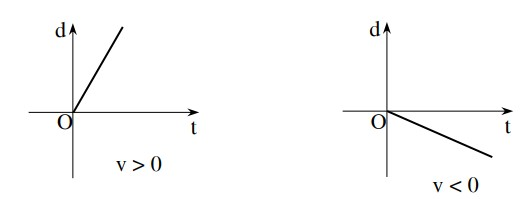
\includegraphics[scale=0.9]{../figs/G10-BAI4-1}
	\end{center}
	* Đồ thị $\left(x-t\right)$ là một đường xiên góc xuất phát từ điểm $\left(x_0;0\right)$. Một số dạng đồ thị sau:
	\begin{center}
		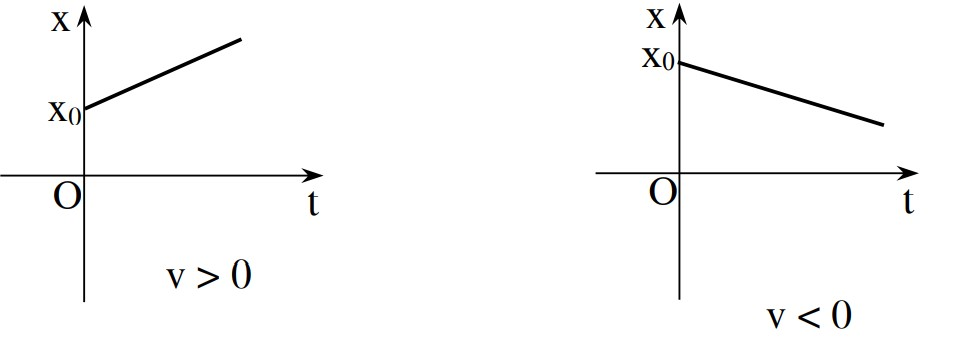
\includegraphics[scale=0.5]{../figs/G10-BAI4-2}
	\end{center}
\end{enumerate}
\subsection{CÁC HỒ SƠ KHÁC}
\textbf{* Các câu hỏi ví dụ}\\
\setcounter{ex}{0}
% ======================================================================
\begin{ex}
	Một chiếc xe đồ chơi đang chuyển động đều trên các đoạn thẳng có độ dịch chuyển tại các thời điểm khác nhau được cho trong bảng dưới đây
	\begin{center}
		\begin{tabular}{|M{3cm}|M{1cm}|M{1cm}|M{1cm}|M{1cm}|M{1cm}|M{1cm}|M{1cm}|M{1cm}|M{1cm}|M{1cm}|M{1cm}|}
			\hline
			\textbf{Thời gian} & 0 & 2 & 4 & 6 & 8 & 10 & 12 & 14 & 16 & 18 & 20\\
			\hline
			\textbf{Độ dịch chuyển $\left(\si{\meter}\right)$} & 0 & 3 & 4 & 4 & 4 & 7 & 10 & 8 & 6 & 4 & 4\\
			\hline
		\end{tabular}
	\end{center}
	\begin{enumerate}[label=\alph*)]
		\item Hãy vẽ đồ thị độ dịch chuyển – thời gian của xe đồ chơi.
		\item Hãy xác định vận tốc và tốc độ tức thời tại các thời điểm $\SI{2}{\second}$, $\SI{6}{\second}$, $\SI{10}{\second}$ và $\SI{16}{\second}$.
		\end{enumerate}
	\loigiai{
	\begin{enumerate}[label=\alph*)]
		\item Đồ thị độ dịch chuyển – thời gian của xe đồ chơi
		\begin{center}
			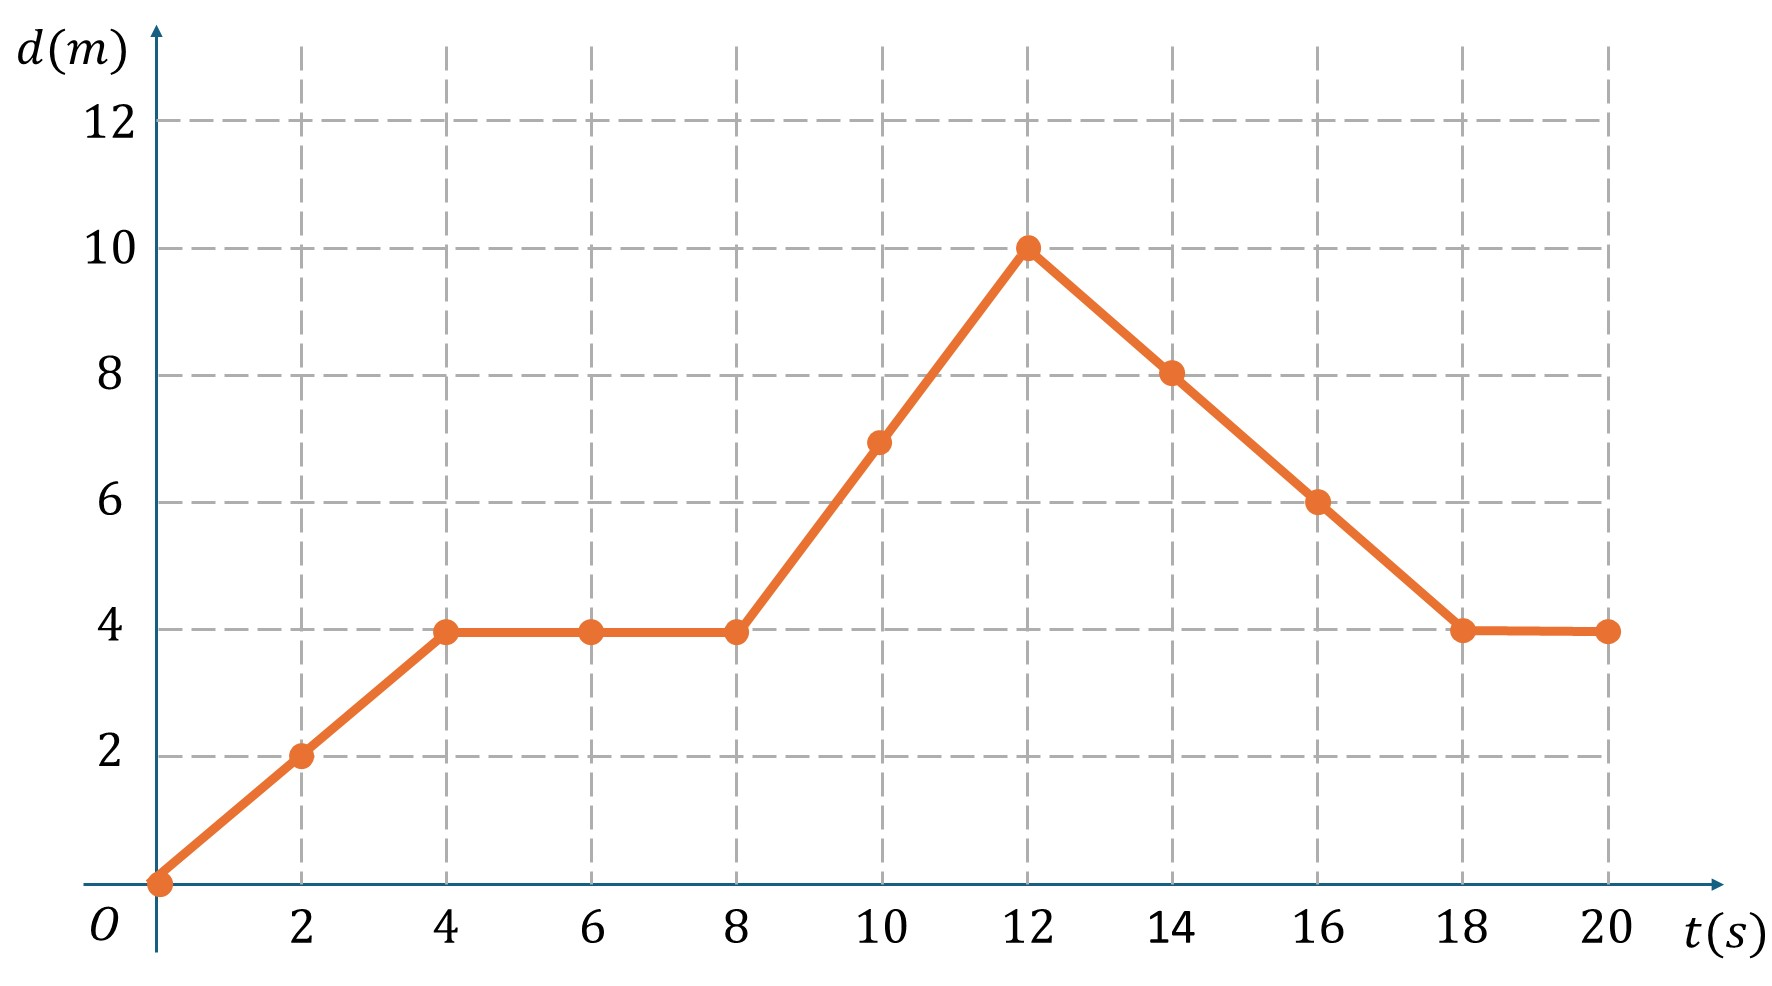
\includegraphics[scale=0.4]{../figs/G10-BAI4-3}
		\end{center}
		\item Vận tốc tức thời và tốc độ tức thời tại các thời điểm:
		\begin{itemize}
			\item $t=\SI{2}{\second}$:\\
			$v=\dfrac{2-0}{2-0}=\SI{1}{\meter/\second}$; $\left|v\right|=\SI{1}{\meter/\second}$.
			\item $t=\SI{6}{\second}$:\\
			$v=\dfrac{4-4}{6-4}=\SI{0}{\meter/\second}$; $\left|v\right|=\SI{0}{\meter/\second}$.
			\item $t=\SI{10}{\second}$:\\
			$v=\dfrac{10-4}{12-8}=\SI{1.5}{\meter/\second}$; $\left|v\right|=\SI{1.5}{\meter/\second}$.
			\item $t=\SI{16}{\second}$:\\
			$v=\dfrac{4-10}{18-12}=\SI{-1}{\meter/\second}$; $\left|v\right|=\SI{1}{\meter/\second}$.
		\end{itemize}
	\end{enumerate}
	}
\end{ex}
% ======================================================================
\begin{ex}
	Phương trình chuyển động của chất điểm dọc theo trục Ox có dạng $x=135-45t$ ($x$ đo bằng kilomet, $t$ đo bằng giờ).
	\begin{enumerate}[label=\alph*)]
		\item Chất điểm xuất phát từ điểm nào? Xác định trạng thái chuyển động của chất điểm.
		\item Xác định vị trí chất điểm tại thời điểm $t=\SI{2}{\hour}$.
		\item Xác định thời điểm chất điểm qua gốc tọa độ.
	\end{enumerate}
	\loigiai{
	\begin{enumerate}[label=\alph*)]
		\item  Chất điểm xuất phát từ điểm có tọa độ $x_0=\SI{135}{\kilo\meter}$ và chuyển động thẳng đều.
		\item Tại thời điểm $t=\SI{2}{\hour}$ thì $x=\SI{45}{\kilo\meter}$.
		\item Chất điểm qua gốc tọa độ thì $x=0\Rightarrow t=\SI{3}{\hour}$.
	\end{enumerate}
	}
\end{ex}
% ======================================================================
\begin{ex}
	Lúc 6 giờ sáng một người đi xe đạp đuổi theo một người đi bộ đã đi được $\SI{8}{\kilo\meter}$. Cả hai chuyển động thẳng đều với các tốc độ lần lượt là $\SI{12}{\kilo\meter/\hour}$ và $\SI{4}{\kilo\meter/\hour}$.
	\begin{enumerate}[label=\alph*)]
		\item Lập phương trình chuyển động của mỗi người trong cùng hệ quy chiếu.
		\item Vẽ đồ thị tọa độ - thời gian của hai người trên cùng hệ trục tọa độ.
		\item Xác định thời điểm và vị trí hai người gặp nhau.
		
	\end{enumerate}
	\loigiai{
	\begin{enumerate}[label=\alph*)]
		\item Chọn gốc tọa độ tại vị trí xuất phát của người đi xe đạp, chiều dương cùng chiều chuyển động của hai người. Gốc thời gian lúc 6 giờ sáng.\\
		Phương trình chuyển động của mỗi người:
		$$\begin{cases}
			x_{\text{xđ}}=12t\\
			x_{\text{b}}=8+4t
		\end{cases}\left(\si{\kilo\meter}; \si{\hour}\right).$$
		\item Vẽ đồ thị tọa độ - thời gian của hai người trên cùng hệ trục tọa độ
		\begin{center}
			\begin{tikzpicture}  
				\begin{axis}[  ultra thick,
					xmin=0,  
					xmax=2.25,  
					xtick={0,0.5,...,2},
					ytick={0,12,24},
					minor x tick num=0,
					minor y tick num=0,
					ymin=0,  
					ymax=28, 
					samples=300,
					axis lines=center, 
					grid style={step=1, line width =0.4pt, color=gray!40!white},
					grid=both, %giới hạn ô lưới
					major grid style={line width=0.8pt,gray!75!white},
					xlabel=$\xsi{t}{\left(\si{\hour}\right)}$, 		ylabel=$\xsi{x}{\left(\si{\kilo\meter}\right)}$,
					every axis y label/.style={at=(current axis.above origin),anchor=south},  
					every axis x label/.style={at=(current axis.right of origin),anchor=west},  ]
					\addplot [line width=1.5pt, red, smooth, domain=0:2] {12*x} node[right] {$x_{\text{xđ}}$}; 
					\addplot [line width=1.5pt, blue, smooth, domain=0:2] {8+4*x} node[right] {$x_{\text{b}}$}; 
					\coordinate (O) at (axis cs: 0,0);
				\end{axis}  
				\node[below left] at (O) {0};
			\end{tikzpicture}
		\end{center}
		\item Dựa vào đồ thị, hai người gặp nhau lúc $t=\SI{1}{\hour}$ tại vị trí cách gốc tọa độ $x=\SI{12}{\kilo\meter}$.
	\end{enumerate}
	}
\end{ex}
\textbf{* Bài tập}\\
\setcounter{ex}{0}
\textbf{BÀI TẬP TRẮC NGHIỆM}
% ===================================================================
\begin{ex}
	Một chiếc xe ô tô xuất phát từ A lúc 6 giờ sáng, chuyển động thẳng đều tới B, cách A $\SI{180}{\kilo\meter}$. Xe tới B lúc 8 giờ 30 phút. Sau 30 phút đỗ tại B, xe chạy ngược về A với tốc độ $\SI{60}{\kilo\meter/\hour}$. Ô tô về tới A lúc
	\choice
	{$\SI{10}{\hour}$}
	{\True $\SI{12}{\hour}$}
	{$\SI{11}{\hour}$}
	{$\SI{10.5}{\hour}$}
	\loigiai{}
\end{ex}
% ===================================================================
\begin{ex}
	Một xe chuyển động thẳng không đổi chiều có tốc độ trung bình là $\SI{20}{\kilo\meter/\hour}$ trên  $\frac{1}{4}$ đoạn đường đầu và $\SI{40}{\kilo\meter/\hour}$ trên $\frac{3}{4}$ đoạn đường còn lại. Tốc độ trung bình của xe trên cả đoạn đường là 	
	\choice
	{$\SI{30}{\kilo\meter/\hour}$}
	{\True $\SI{32}{\kilo\meter/\hour}$}
	{$\SI{26.67}{\kilo\meter/\hour}$}
	{$\SI{35}{\kilo\meter/\hour}$}
	\loigiai{}
\end{ex}
% ===================================================================
\begin{ex}
	Một chất điểm chuyển động dọc theo trục $Ox$ có phương trình tọa độ $x=4-10t$ trong đó $x$ tính theo đơn vị $\si{\kilo\meter}$ và $t$ tính theo đơn vị giờ. Quãng đường đi được của chất điểm sau 2 giờ chuyển động là
	\choice
	{$\SI{8}{\kilo\meter}$}
	{$\SI{16}{\kilo\meter}$}
	{\True $\SI{20}{\kilo\meter}$}
	{$\SI{12}{\kilo\meter}$}
	\loigiai{}
\end{ex}
% ===================================================================
\begin{ex}
	Cho đồ thị tọa độ - thời gian của một chiếc xe chuyển động thẳng như hình bên dưới. 
	\begin{center}
		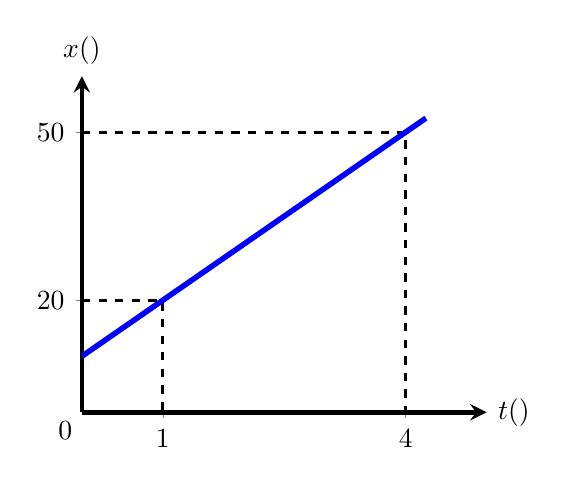
\begin{tikzpicture}  
			\begin{axis}[  ultra thick,scale=0.75,
				xmin=0,  
				xmax=5,  
				xtick={0,1,4},
				ytick={0,20,50},
				minor x tick num=0,
				minor y tick num=0,
				ymin=0,  
				ymax=60, 
				samples=300,
				axis lines=center, 
				xlabel=$\xsi{t}{\left(\si{\hour}\right)}$, 		ylabel=$\xsi{x}{\left(\si{\kilo\meter}\right)}$,
				every axis y label/.style={at=(current axis.above origin),anchor=south},  
				every axis x label/.style={at=(current axis.right of origin),anchor=west},  ]
				\draw[dashed, line width=1pt] (axis cs: 0,20)--(axis cs:1,20)--(axis cs:1,0);
				\draw[dashed, line width=1pt] (axis cs:0,50)--(axis cs:4,50)--(axis cs:4,0);
				\addplot [line width=2pt, blue, smooth, domain=0:4.25] {20+10*(x-1)};  
				\coordinate (O) at (axis cs: 0,0);
			\end{axis}  
			\node[below left] at (O) {0};
		\end{tikzpicture}
	\end{center}
	Phương trình tọa độ của xe là
	
	\choice
	{$x=15+5t$}
	{\True $x=10+10t$}
	{$x=20+10t$}
	{$x=-10+15t$}
	\loigiai{}
\end{ex}
% ===================================================================
\begin{ex}
	Đồ thị độ dịch chuyển – thời gian của một vật chuyển động như hình vẽ. Vật chuyển động
	\begin{center}
		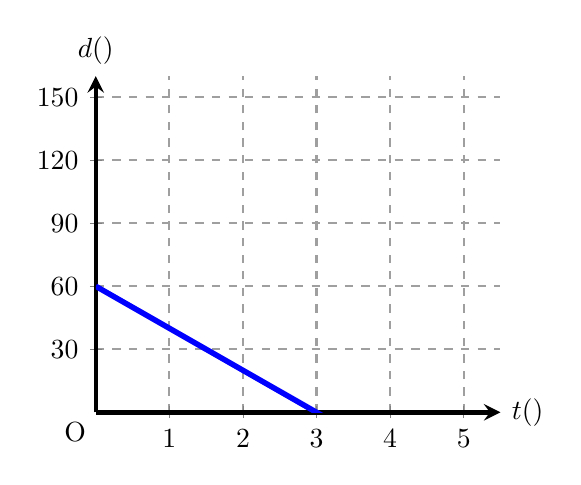
\begin{tikzpicture}  
			\begin{axis}[  ultra thick, scale=0.75,
				xmin=0,  
				xmax=5.5,  
				xtick={0,1,...,5},
				ytick={0,30,...,150},
				minor x tick num=0,
				minor y tick num=0,
				ymin=0,  
				ymax=160, 
				samples=300,
				axis lines=center, 
				grid style={step=1, line width =0.4pt, color=gray!40!white},
				grid=both, %giới hạn ô lưới
				major grid style={line width=0.8pt,gray!75!white, dashed},
				xlabel=$\xsi{t}{\left(\si{\hour}\right)}$, 		ylabel=$\xsi{d}{\left(\si{\kilo\meter}\right)}$,
				every axis y label/.style={at=(current axis.above origin),anchor=south},  
				every axis x label/.style={at=(current axis.right of origin),anchor=west},  ]
				\addplot [line width=2pt, blue, smooth, domain=0:5] {60-20*x};  
				\coordinate (O) at (axis cs: 0,0);
			\end{axis}  
			\node[below left] at (O) {O};
		\end{tikzpicture}
	\end{center}
	\choice
	{cùng chiều dương với tốc độ $\SI{60}{\kilo\meter/\hour}$}
	{\True ngược chiều dương với tốc độ $\SI{20}{\kilo\meter/\hour}$}
	{cùng chiều dương với tốc độ $\SI{20}{\kilo\meter/\hour}$}
	{ngược chiều dương với tốc độ $\SI{60}{\kilo\meter/\hour}$}
	\loigiai{}
\end{ex}
% ===================================================================
\begin{ex}
	Kết luận nào sau đây là \textbf{đúng} khi nói về độ dịch chuyển và quãng đường đi được của một vật?	
	\choice
	{Độ dịch chuyển và quãng đường đi được đều là đại lượng vô hướng}
	{\True Độ dịch chuyển là đại lượng vector còn quãng đường đi được là đại lượng vô hướng}
	{Độ dịch chuyển và quãng đường đi được đều là đại lượng vector}
	{Độ dịch chuyển và quãng đường đi được đều là đại lượng không âm}
	\loigiai{}
\end{ex}
% ===================================================================
\begin{ex}
	Khi vật chuyển động thẳng đều cùng chiều dương thì đồ thị $d - t$ của vật có dạng là
	\choice
	{đường thẳng vuông góc với trục $Od$}
	{\True đường thẳng xiên góc đi lên}
	{đường thẳng xiên góc đi xuống}
	{đường thẳng vuông góc với trục $Ot$}
	\loigiai{}
\end{ex}
%% ===================================================================
%\begin{ex}
%	Cho đồ thị độ dịch chuyển – thời gian của một vật như hình. Chọn phát biểu \textbf{đúng}.	
%	\begin{center}
%		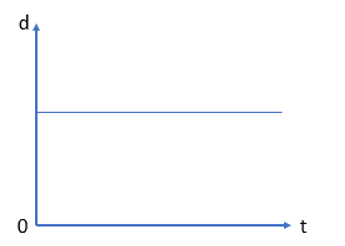
\includegraphics[width=0.25\linewidth]{figs/VN10-2023-PH-TP005-P-1}
%	\end{center}
%	\choice
%	{Vật đang chuyển động thẳng đều theo chiều dương}
%	{Vật đang chuyển động thẳng đều theo chiều âm}
%	{\True Vật đang đứng yên}
%	{Vật chuyển động thẳng đều theo chiều dương rồi đổi chiều chuyển động ngược lại}
%	\loigiai{}
%\end{ex}

% ===================================================================
\begin{ex}
	Một vật bắt đầu chuyển động từ điểm O đến điểm A, sau đó chuyển động về điểm B. Quãng đường và độ dịch chuyển của vật tương ứng là	
	\begin{center}
		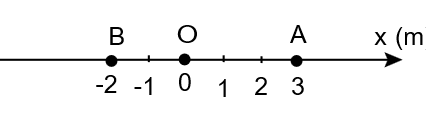
\includegraphics[width=0.4\linewidth]{figs/VN10-2022-PH-TP004-P-2}
	\end{center}
	\choice
	{$\SI{2}{\meter}$; $\SI{-2}{\meter}$}
	{\True $\SI{8}{\meter}$; $\SI{-2}{\meter}$}
	{$\SI{2}{\meter}$; $\SI{2}{\meter}$}
	{$\SI{8}{\meter}$; $\SI{-8}{\meter}$}
	\loigiai{}
\end{ex}
% ===================================================================
\begin{ex}
	“Lúc 15 giờ 30 phút hôm qua, xe chúng tôi đang chạy trên quốc lộ 5, cách Hải Dương 10 km”. Việc xác định vị trí của ô tô như trên còn thiếu yếu tố gì?	
	\choice
	{Vật làm mốc}
	{\True Chiều dương trên đường đi}
	{Mốc thời gian}
	{Thước đo và đồng hồ}
	\loigiai{}
\end{ex}

% ===================================================================
\begin{ex}
	
	Hai người đi xe đạp từ A đến C, người thứ nhất đi theo đường từ A đến B, rồi từ B đến C; người thứ hai đi thẳng từ A đến C. Cả hai đều về đích cùng một lúc.\\
	Hãy chọn kết luận \textbf{sai}.	
	\immini{
		\choice
		{Người thứ nhất đi được quãng đường $\SI{8}{\kilo\meter}$}
		{Độ dịch chuyển của người thứ nhất và người thứ hai bằng nhau}
		{\True Độ dịch chuyển và quãng đường đi được của người thứ nhất bằng nhau}
		{Độ dịch chuyển của người thứ nhất là $\SI{5.7}{\kilo\meter}$, hướng $\SI{45}{\degree}$ Đông – Bắc}
	}
	{
		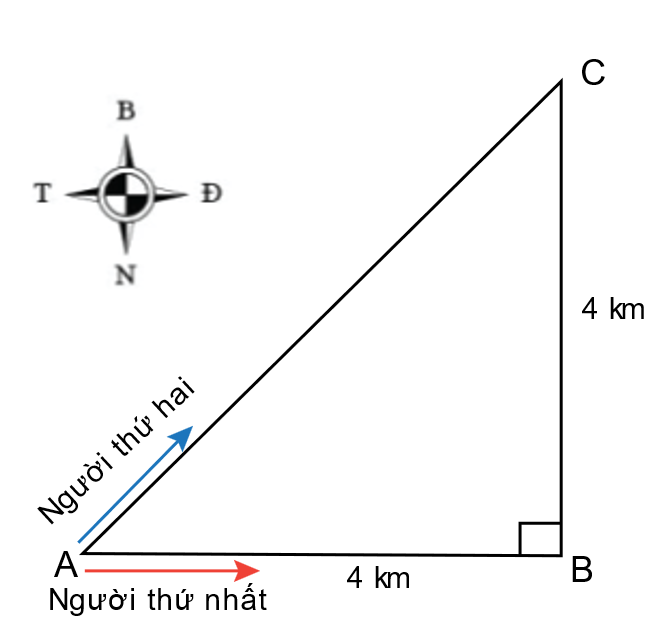
\includegraphics[width=0.5\linewidth]{figs/VN10-2022-PH-TP004-P-3}
	}
	\loigiai{}
	
\end{ex}
% ===================================================================
\begin{ex}
	Khi nhìn vào tốc kế của ô tô đang chạy, số chỉ trên tốc kế cho ta biết
	\choice
	{gia tốc tức thời của ô tô}
	{vận tốc tức thời của ô tô}
	{\True tốc độ tức thời của ô tô}
	{tốc độ trung bình của ô tô}
	\loigiai{}
\end{ex}
% ===================================================================
\begin{ex}
	Một máy bay phản lực có tốc độ $\SI{700}{\kilo\meter/\hour}$. Nếu muốn bay liên tục trên khoảng cách $\SI{1400}{\kilo\meter}$ thì máy bay phải bay trong thời gian là
	\choice
	{\True $\SI{2}{\hour}$}
	{$\SI{3}{\hour}$}
	{$\SI{2}{\hour}\SI{30}{\minute}$}
	{$\SI{1}{\hour}\SI{30}{\minute}$}
	\loigiai{Thời gian máy bay bay quãng đường $\SI{1400}{\kilo\meter}$:
		$$t=\dfrac{s}{v}=\SI{2}{\hour}.$$}
\end{ex}
% ===================================================================
\begin{ex}
	Đồ thị độ dịch chuyển – thời gian trong chuyển động thẳng của một chất điểm có dạng như hình vẽ.\\
	Trong thời gian nào xe chuyển động thẳng đều?
	\begin{center}
		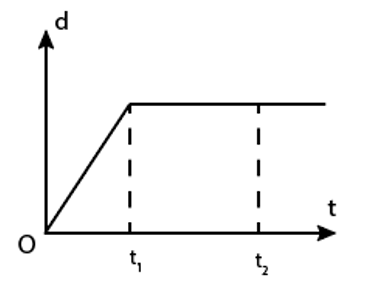
\includegraphics[width=0.25\linewidth]{figs/VN10-2023-PH-TP005-P-4}
	\end{center}
	\choice
	{\True Trong khoảng thời gian từ $0$ đến $t_1$}
	{Trong khoảng thời gian từ $0$ đến $t_2$}
	{Trong khoảng thời gian từ $t_1$ đến $t_2$}
	{Không có lúc nào xe chuyển động thẳng đều}
	\loigiai{}
\end{ex}
% ===================================================================
\begin{ex}
	Phương trình chuyển động của một chất điểm dọc theo trục $Ox$ có dạng: $x = 5 + 60t$ ($x$ đo bằng kilomét và $t$ đo bằng giờ). Chất điểm đó xuất phát từ điểm nào và chuyển động với vận tốc bằng bao nhiêu?
	\choice
	{Từ điểm $O$, với vận tốc $\SI{5}{\kilo\meter/\hour}$}
	{Từ điểm $O$, với vận tốc $\SI{60}{\kilo\meter/\hour}$}
	{Từ điểm cách $O$ $\SI{5}{\kilo\meter/\hour}$, với vận tốc $\SI{5}{\kilo\meter/\hour}$}
	{\True Từ điểm cách $O$ $\SI{5}{\kilo\meter/\hour}$, với vận tốc $\SI{60}{\kilo\meter/\hour}$}
	\loigiai{}
\end{ex}
% ===================================================================
\begin{ex}
	Phương trình chuyển động của một chất điểm dọc theo $Ox$ có dạng: $x=5t-12$ (km), với $t$ đo bằng giờ. Độ dịch chuyển của chất điểm từ $\SI{2}{\hour}$ đến $\SI{4}{\hour}$ là	
	\choice
	{$\SI{8}{\kilo\meter}$}
	{$\SI{6}{\kilo\meter}$}
	{\True $\SI{10}{\kilo\meter}$}
	{$\SI{2}{\kilo\meter}$}
	\loigiai{}
\end{ex}
% ===================================================================
\begin{ex}
	Phương trình chuyển động của một chất điểm dọc theo trục $Ox$ có dạng: $x = 4 -10t$ ($x$ đo bằng kilomét và $t$ đo bằng giờ). Quãng đường đi được của chất điểm sau $\SI{2}{\hour}$ chuyển động là
	\choice
	{$\SI{-20}{\kilo\meter}$}
	{\True $\SI{20}{\kilo\meter}$}
	{$\SI{-8}{\kilo\meter}$}
	{$\SI{8}{\kilo\meter}$}
	\loigiai{}
\end{ex}

% ===================================================================
\begin{ex}
	Một xe xuất phát từ lúc 7 giờ 15 phút sáng từ thành phố M, chuyển động thẳng đều tới thành phố N, cách thành phố M $\SI{90}{\kilo\meter}$. Biết tốc độ của xe là $\SI{60}{\kilo\meter/\hour}$, xe đến thành phố N lúc
	\choice
	{9 giờ 45 phút}
	{8 giờ 30 phút}
	{9 giờ 30 phút}
	{\True 8 giờ 45 phút}
	\loigiai{Thời gian để xe đi từ M đến N:
		$$\Delta t=\dfrac{s}{v}=\SI{1.5}{\hour}.$$
		Thời điểm xe đến N:
		$$t=\SI{7}{\hour}\SI{15}{\minute}+\Delta t=\SI{8}{\hour}\SI{45}{\minute}.$$}
\end{ex}
% ===================================================================
\begin{ex}
	Trong nội dung thi đấu môn bơi ếch $\SI{100}{\meter}$, một vận động viên đã hoàn thành đường đua với thành tích $\SI{63.25}{\second}$. Tốc độ trung bình của vận động viên này trong giải thi đấu đó là bao nhiêu?
	\choice
	{\True $\SI{1.58}{\meter/\second}$}
	{$\SI{0.63}{\meter/\second}$}
	{$\SI{6.33}{\meter/\second}$}
	{$\SI{36.75}{\meter/\second}$}
	\loigiai{ Tốc độ trung bình của vận động viên này
		$$v_\text{tb}=\dfrac{s}{t}\approx\SI{1.58}{\meter/\second}.$$}
\end{ex}
% ===================================================================
\begin{ex}
	Một ô tô chạy thử nghiệm trên một đoạn đường thẳng. Cứ $\SI{5}{\second}$ thì có một giọt dầu từ động cơ của ô tô rơi thẳng xuống mặt đường. Hình bên cho thấy mô hình các giọt dầu để lại trên mặt đường. Ô tô chuyển động trên đường này với tốc độ trung bình là
	\begin{center}
		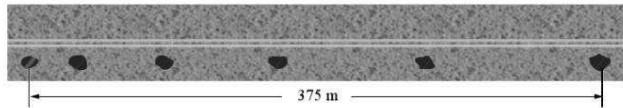
\includegraphics[width=0.5\linewidth]{figs/VN10-2022-PH-TP004-1-P-1}
	\end{center}	
	\choice
	{$\SI{12.5}{\meter/\second}$}
	{\True $\SI{15}{\meter/\second}$}
	{$\SI{30}{\meter/\second}$}
	{$\SI{25}{\meter/\second}$}
	\loigiai{Tốc độ trung bình của ô tô:
		$$v_\text{tb}=\dfrac{s}{t}=\dfrac{\SI{375}{\meter}}{\SI{25}{\second}}=\SI{15}{\meter/\second}.$$}
\end{ex}
% ===================================================================
\begin{ex}
	Một xe chuyển động thẳng không đổi chiều, $\SI{1}{\hour}$ đầu xe chạy với tốc độ trung bình $\SI{60}{\kilo\meter/\hour}$ và $\SI{3}{\hour}$ sau xe chạy với tốc độ trung bình $\SI{40}{\kilo\meter/\hour}$. Tốc độ trung bình của xe trong suốt thời gian chuyển động là
	\choice
	{$\SI{48}{\kilo\meter/\hour}$}
	{$\SI{40}{\kilo\meter/\hour}$}
	{$\SI{58}{\kilo\meter/\hour}$}
	{\True $\SI{45}{\kilo\meter/\hour}$}
	\loigiai{$$v_{tb}=\dfrac{v_1t_1+v_2t_2}{t_1+t_2}=\SI{45}{\kilo\meter/\hour}.$$}
\end{ex}
% ===================================================================
\begin{ex}
	Một người đi xe đạp trên $\dfrac{2}{3}$ đoạn đường đầu với tốc độ trung bình $\SI{10}{\kilo\meter/\hour}$ và $\dfrac{1}{3}$ đoạn đường sau với tốc độ trung bình $\SI{20}{\kilo\meter/\hour}$. Tốc độ trung bình của người đi xe đạp trên cả quãng đường là
	\choice
	{\True $\SI{12}{\kilo\meter/\hour}$}
	{$\SI{15}{\kilo\meter/\hour}$}
	{$\SI{17}{\kilo\meter/\hour}$}
	{$\SI{13.3}{\kilo\meter/\hour}$}
	\loigiai{Gọi $s$ là chiều dài đoạn đường
		$$v_{tb}=\dfrac{s}{t_1+t_2}=\dfrac{s}{\dfrac{2s}{3v_1}+\dfrac{s}{3v_2}}=\dfrac{1}{\dfrac{2}{3v_1}+\dfrac{1}{3v_2}}=\SI{12}{\kilo\meter/\hour}.$$}
\end{ex}
% ===================================================================
\begin{ex}
	Hình vẽ bên là đồ thị độ dịch chuyển - thời gian của một chiếc xe ô tô chạy từ $A$ đến $B$ trên một đường thẳng. Vận tốc của xe bằng
	\begin{center}
		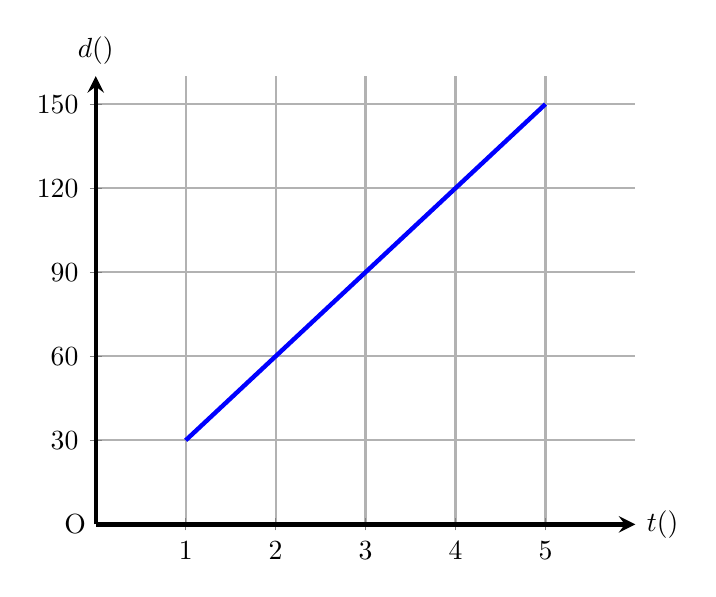
\begin{tikzpicture}  
			\begin{axis}[  ultra thick,
				xmin=0,  
				xmax=6,  
				xtick={0,1,...,5},
				ytick={0,30,...,150},
				minor x tick num=0,
				minor y tick num=0,
				ymin=0,  
				ymax=160, 
				samples=300,
				axis lines=center, 
				grid style={step=1, line width =0.4pt, color=gray!30!white},
				grid=both,
				major grid style={line width=0.8pt,gray!60!white},
				xlabel=$\xsi{t}{\left(\si{\hour}\right)}$, 		ylabel=$\xsi{d}{\left(\si{\kilo\meter}\right)}$,
				every axis y label/.style={at=(current axis.above origin),anchor=south},  
				every axis x label/.style={at=(current axis.right of origin),anchor=west},  ]
				\addplot [ultra thick, blue, smooth, domain=1:5] {30*x};			 
			\end{axis}  
			\node[left] at (0,0) {O};
		\end{tikzpicture}
	\end{center}
	\choice
	{\True $\SI{30}{\kilo\meter/\hour}$}
	{$\SI{150}{\kilo\meter/\hour}$}
	{$\SI{120}{\kilo\meter/\hour}$}
	{$\SI{100}{\kilo\meter/\hour}$}
	\loigiai{}
\end{ex}
% ===================================================================
\begin{ex}
	Một chất điểm chuyển động trên một đường thẳng. Đồ thị độ dịch chuyển theo thời gian của chất điểm được mô tả như hình vẽ. Tốc độ trung bình của chất điểm trong khoảng thời gian từ 0 đến $\SI{5}{\second}$ là
	\begin{center}
		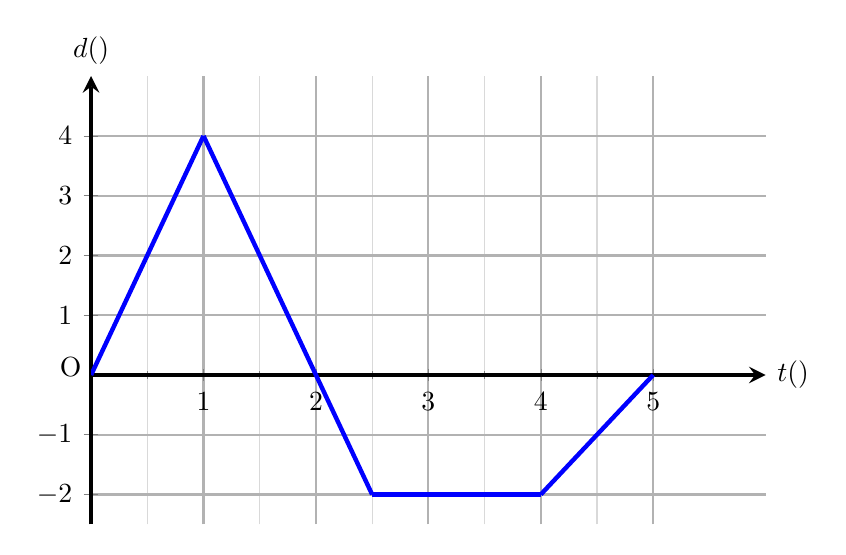
\begin{tikzpicture}  
			\begin{axis}[  ultra thick,xscale=1.25,
				xmin=0,  
				xmax=6,  
				xtick={0,1,...,5},
				ytick={-2,-1,0,1,...,4},
				minor x tick num=1,
				minor y tick num=0,
				ymin=-2.5,  
				ymax=5, 
				samples=300,
				axis lines=center, 
				grid style={step=1, line width =0.4pt, color=gray!30!white},
				grid=both,
				major grid style={line width=0.8pt,gray!60!white},
				xlabel=$\xsi{t}{\left(\si{\second}\right)}$, 		ylabel=$\xsi{d}{\left(\si{\centi\meter}\right)}$,
				every axis y label/.style={at=(current axis.above origin),anchor=south},  
				every axis x label/.style={at=(current axis.right of origin),anchor=west},  ]
				\addplot [ultra thick, blue, smooth, domain=0:1] {4*x};	
				\addplot [ultra thick, blue, smooth, domain=1:2.5] {4-4*(x-1)};		
				\addplot [ultra thick, blue, smooth, domain=2.5:4] {-2};	 
				\addplot [ultra thick, blue, smooth, domain=4:5] {-2+2*(x-4)};
				
			\end{axis}  
			\node[left] at (0,2) {O};
			
		\end{tikzpicture}
	\end{center}
	\choice
	{$\SI{1.6}{\centi\meter/\second}$}
	{$\SI{6.4}{\centi\meter/\second}$}
	{$\SI{4.8}{\centi\meter/\second}$}
	{\True $\SI{2.4}{\centi\meter/\second}$}
	\loigiai{
		Tốc độ trung bình của chất điểm:
		$$v_\text{tb}=\dfrac{s}{t}=\dfrac{4+4+2+2}{5}=\SI{2.4}{\centi\meter/\second}.$$	
	}
\end{ex}
% ===================================================================
\begin{ex}
	Đồ thị toạ độ - thời gian của hai xe (I) và (II) cùng chuyển động trên một đường thẳng được thể hiện như hình bên. Thời điểm hai xe gặp nhau là
	\begin{center}
		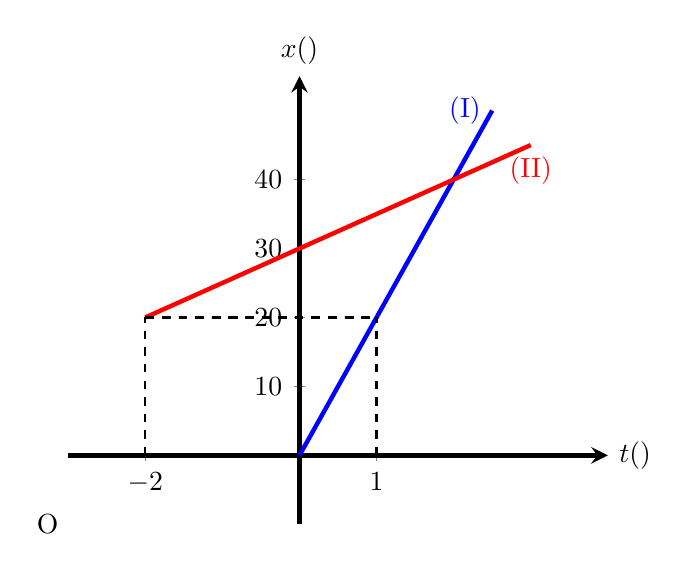
\begin{tikzpicture}  
			\begin{axis}[  ultra thick,
				xmin=-3,  
				xmax=4,  
				xtick={-2,0,1},
				ytick={0,10,...,40},
				minor x tick num=0,
				minor y tick num=0,
				ymin=-10,  
				ymax=55, 
				samples=300,
				axis lines=center, 
				xlabel=$\xsi{t}{\left(\si{\hour}\right)}$, 		ylabel=$\xsi{x}{\left(\si{\kilo\meter}\right)}$,
				every axis y label/.style={at=(current axis.above origin),anchor=south},  
				every axis x label/.style={at=(current axis.right of origin),anchor=west},  ]
				\addplot [ultra thick, blue, smooth, domain=0:2.5] {20*x} node[left] {(I)};	
				\addplot [ultra thick, red, smooth, domain=-2:3] {30+5*x} node[below] {(II)};	
				\addplot [thick, dashed, domain=-2:1] {20} ;	
				\draw[thick, dashed] (axis cs:-2,0) --(axis cs:-2,20);	 
				\draw[thick, dashed] (axis cs:1,0) --(axis cs: 1,20);
			\end{axis}  
			\node[left] at (0,0) {O};
		\end{tikzpicture}
	\end{center}
	\choice
	{$\SI{1}{\hour}$}
	{\True$\SI{2}{\hour}$}
	{$\SI{2.5}{\hour}$}
	{$\SI{1.33}{\hour}$}
	\loigiai{}
\end{ex}

% ===================================================================
\begin{ex}
	Hình dưới là đồ thị độ dịch chuyển - thời gian của hai vật chuyển động thẳng cùng hướng. Tỉ lệ vận tốc $\dfrac{v_A}{v_B}$ là
	\begin{center}
		\begin{tikzpicture} 
			\coordinate (O)  at (0,0);
			\coordinate (t) at (4,0);
			\coordinate (d) at (0,4);
			\coordinate (A) at ($(O)+(30:3)$);
			\coordinate (B) at ($(O)+(60:3.5)$);
			\draw[line width=1pt, -latex] (O)--(d);
			\draw[line width=1pt, -latex] (O)--(t);
			\draw[line width=1.5pt, red] (O)--(A);
			\draw[line width=1.5pt, blue] (O)--(B);
			\node[left] at (O) {O};
			\node[above] at (t) {$t$};
			\node[left] at (d) {$d$};
			\tkzFillAngle[size=0.75cm,color=red, fill=red, opacity=0.25](t,O,A);
			\tkzLabelAngle[color=red,pos=1.2](t,O,A){$\SI{30}{\degree}$}
			\tkzMarkAngle[size=0.5cm,color=blue](t,O,B);
			\node[blue] at (0.75,0.7) {$\SI{60}{\degree}$};
		\end{tikzpicture}
	\end{center}
	\choice
	{$\dfrac{3}{1}$}
	{$\dfrac{1}{3}$}
	{$\dfrac{\sqrt{3}}{1}$}
	{$\dfrac{1}{\sqrt{3}}$}
	\loigiai{}
\end{ex}
\textbf{BÀI TẬP TỰ LUẬN}
% ======================================================================
\begin{ex}
	Lúc $\SI{7}{\hour}$ có một xe khởi hành từ A chuyển động thẳng đều về B với tốc độ $\SI{40}{\kilo\meter/\hour}$. Lúc $\SI{7}{\hour}\SI{30}{\minute}$ một xe khác khởi hành từ B chuyển động thẳng đều về A  với tốc độ $\SI{50}{\kilo\meter/\hour}$. Cho $\mathrm{AB}=\SI{110}{\kilo\meter}$.
	\begin{enumerate}[label=\alph*)]
		\item Xác định vị trí của mỗi xe và khoảng cách giữa chúng lúc $\SI{8}{\hour}$ và lúc $\SI{9}{\hour}$.
		\item Hai xe gặp nhau lúc mấy giờ? Ở đâu?
	\end{enumerate}
	\loigiai{
		\begin{enumerate}[label=\alph*)]
			\item Cách A $\SI{40}{\kilo\meter}$, $\SI{85}{\kilo\meter}$, $\SI{45}{\kilo\meter}$.\\
			Cách A $\SI{80}{\kilo\meter}$, $\SI{35}{\kilo\meter}$, $\SI{45}{\kilo\meter}$.
			\item $\SI{8}{\hour}\SI{30}{\minute}$; cách A $\SI{60}{\kilo\meter}$.
		\end{enumerate}
	}
\end{ex}
% ======================================================================
\begin{ex}
	Hai xe chuyển động trên hai đường vuông góc với nhau, xe A đi về hướng tây với tốc độ $\SI{50}{\kilo\meter/\hour}$, xe B đi về hướng Nam với tốc độ $\SI{30}{\kilo\meter/\hour}$. Vào một thời điểm nào đó xe A và B còn cách giao điểm của hai đường lần lượt là $\SI{4.4}{\kilo\meter}$ và $\SI{4}{\kilo\meter}$, hai xe đang tiến về phía giao điểm. Tìm khoảng cách ngắn nhất giữa hai xe.
	\loigiai{
		$\SI{1.166}{\kilo\meter}$.
	}
\end{ex}